\chapter{Diseño}
\label{chap:diseño}

En este capítulo de la memoria vamos a describir los diagramas de clases para la base de datos y también el diagrama de flujo para el entorno BackEnd y FrontEnd. Para ello empezaremos por definir el diagrama de la base de datos.

\section{Clases de la BD}

\begin{figure}[H]
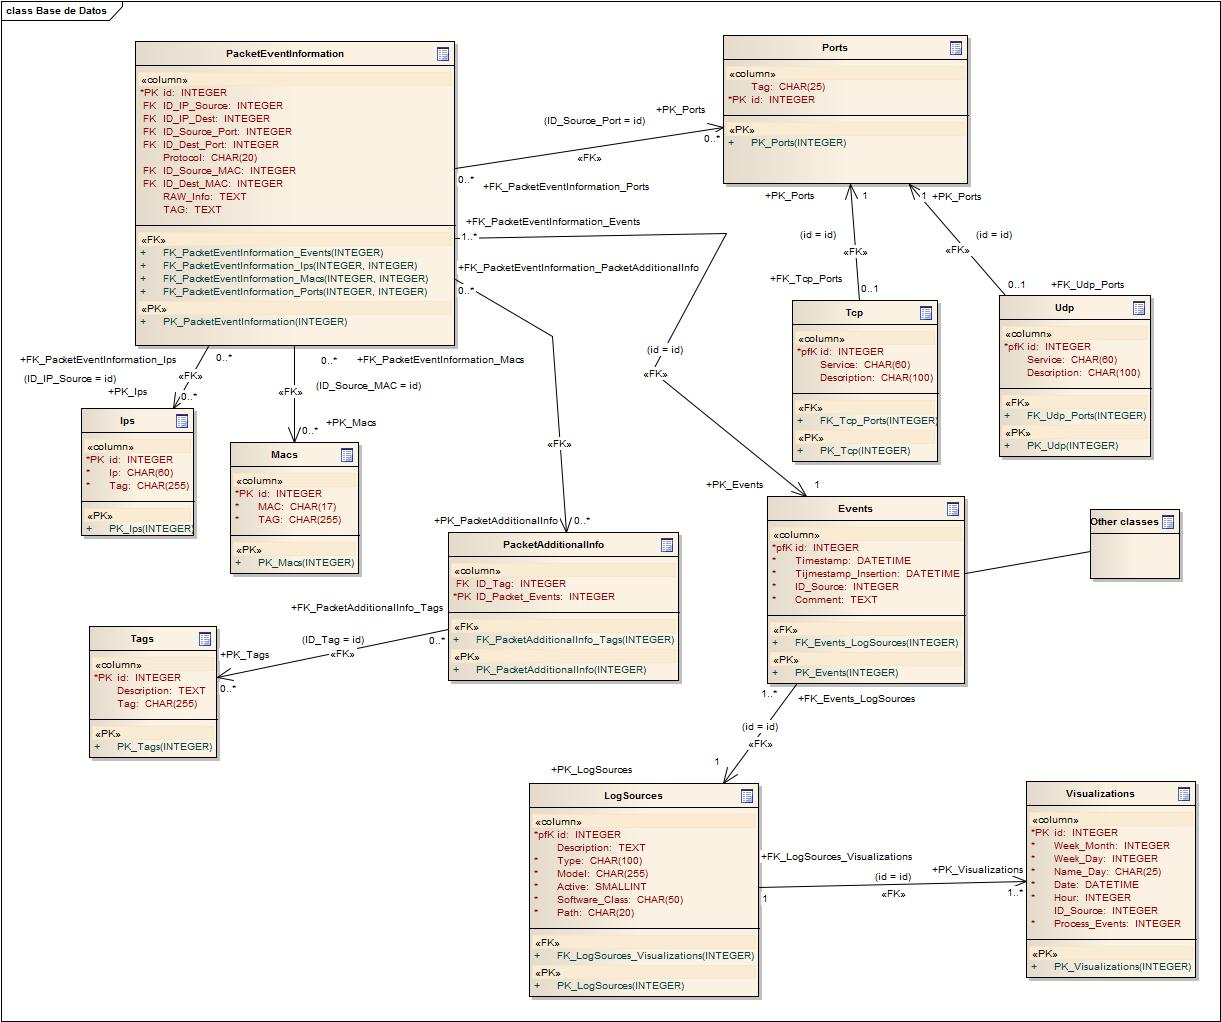
\includegraphics[scale=.35]{diagramas/bd.jpg}
\caption{Diagrama de clases para la BD (usando ORM)}
\end{figure}

La clase o tabla que contendrá el peso de toda la jerarquía de base de datos, será \textbf{PacketEventsInformation}. Esta tabla sólo contendrá referencias externas o ``foreign keys'' a cada tabla que haga participe en su definición, es decir:
\begin{itemize}
\item Ips
\item Macs
\item Ports
\item Events
\item PacketAdditionalInfo
\end{itemize}

Cómo podemos observar en el diagrama anterior, por ejemplo, para la clase PacketEventInformation, tenemos su traducción a formato ORM del motor proporcionado por Django:

\begin{figure}[H]
\lstinputlisting{trozos-codigo/codigo-8.py}
\caption{Ejemplo de clase ORM, en concreto PacketEventsInformation}
\end{figure}

\section{Flujo de ejecución de la aplicación}

Ahora toca la parte de diagramas de secuencias para la interacción entre el usuario y el procesamiento de fuentes (Back); y el usuario y la visualización de los datos en la web de la aplicación (Front).\\
\pagebreak
\subsection{BackEnd}

\begin{figure}[h]
\vspace*{-5in}{\hspace*{-.3in}{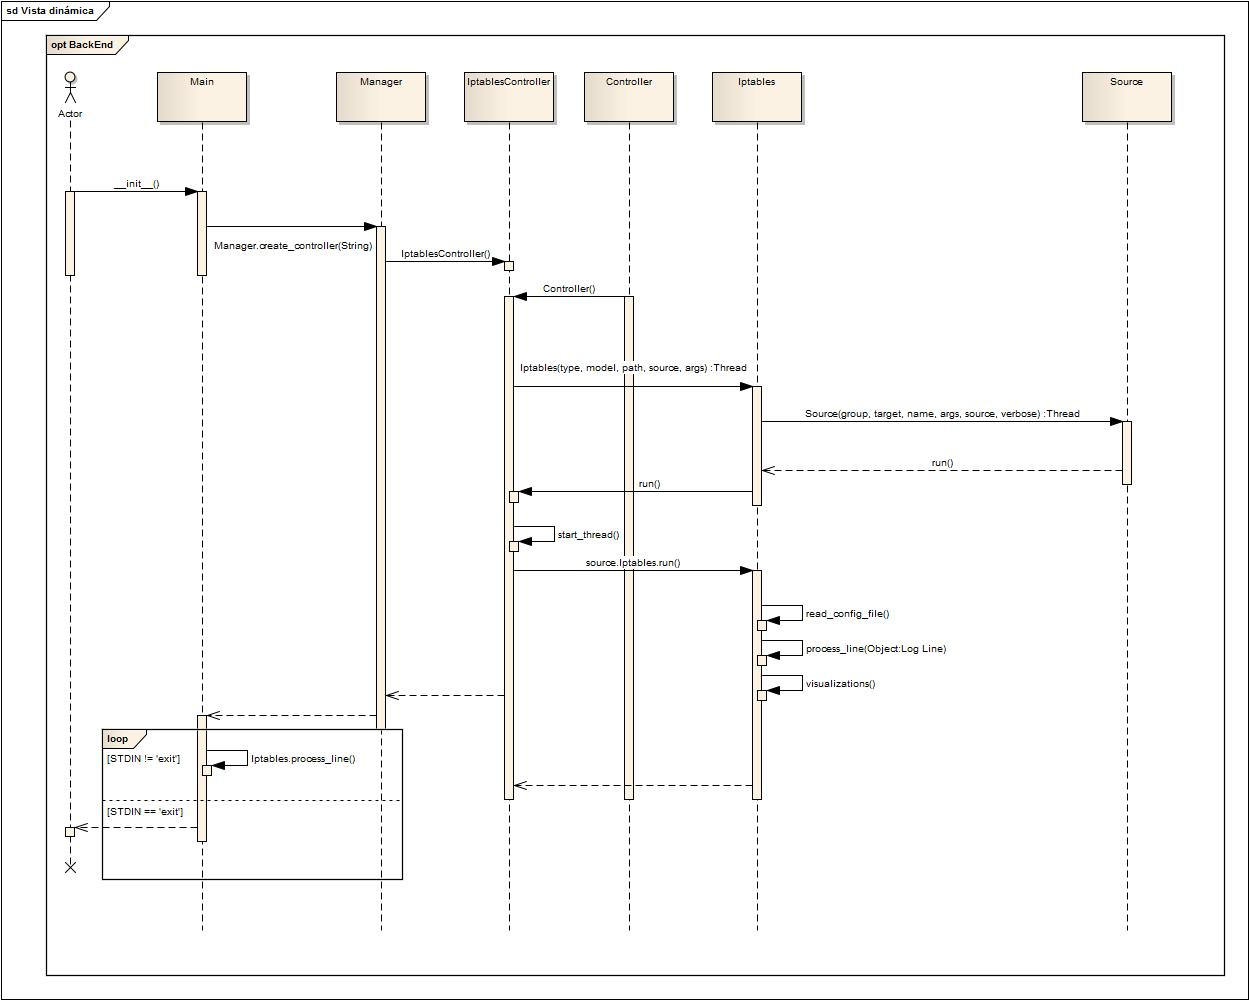
\includegraphics[scale=.4]{diagramas/secuencia-back.jpg}}}
\caption{Diagrama de Secuencia para la parte BackEnd}
\end{figure}

\pagebreak

\subsection{FrontEnd}

\begin{figure}[H]
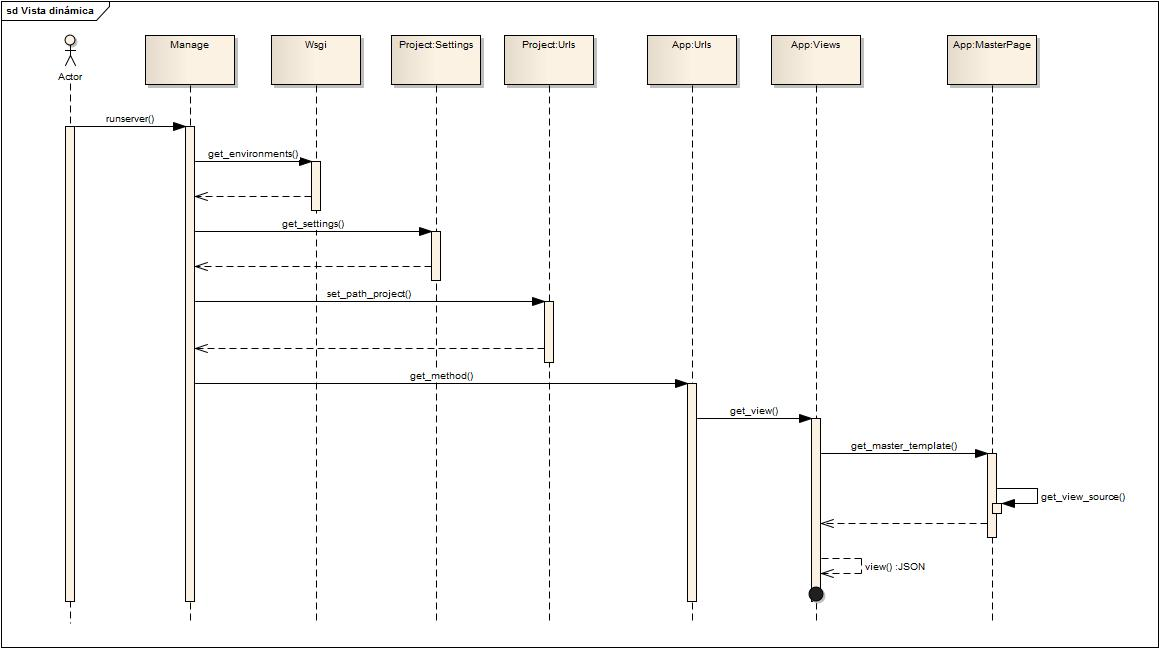
\includegraphics[scale=.4]{diagramas/secuencia-front.jpg}
\caption{Diagrama de Secuencia para la parte FrontEnd}
\end{figure}

[TODO]

\begin{itemize}
\item estructura de clases (diagrama)
\item diseño de la vista (patrón)
\item arquitectura del sistema 
\end{itemize}

[TODO]
